\documentclass[paper=a4, fontsize=11pt]{scrartcl}
\usepackage{hyperref}
\usepackage{listings}
\usepackage{cite}
\usepackage{booktabs} % Required for better horizontal rules in tables
\usepackage{multirow}
\usepackage{multicol}
\usepackage{graphicx}

\lstset{
	sensitive=false,    % not case-sensitive
	morecomment=[l]{;;}, % line comment
	alsoletter={:,-},   % consider extra characters
	frame=single,
	numbers=left,
	breaklines=true,
	tabsize=2,
	basicstyle=\footnotesize,
}

\setlength\parindent{0pt}

\title{Project: Storing Groceries @home}
\author{\'{A}ngela Patricia Enr\'{i}quez G\'{o}mez \\
	Ethan Massey \\
	Maximilian Messing}

\begin{document}

	\maketitle

 	\section{Introduction}

 	This project creates plans for storing groceries tasks in the context of RoboCup @home. It uses the java version of the SHOP2 HTN Planner. \\

 	The robot picks up groceries from a table and stores them in a cupboard with 3 shelves. The door of the cupboard is closed at the beginning,
 	and the robot has a tray to carry more than one item at a time.

 	\section{Selection of the Planner}

 	SHOP2 (Simple Hierarchical Ordered Planner) is an HTN Planner that uses partial-order forward decomposition. SHOP2 does not require methods to be totally ordered, i.e., the subtasks of a method can have partial orders. Because of this property, SHOP2 can generate plans by interleaving tasks of different methods. Its predecessor SHOP can only handle methods with totally ordered subtasks and thus, is more limited in the plans it can generate. SHOP can overcome this limitation by adding global methods that allow to perform more general actions \cite{Nau2001}, like adding a pick-two-object method instead of just having a pick-one-object method. However, SHOP2 can interleave the tasks of two pick-one-object methods in such a way that it gives the same results as the more global method pick-two-objects \cite{slides}. \\

 	With SHOP2 the knowledge base is easier to build, because it requires less global information. Having more compact knowledge bases makes it faster to generate them and easier to debug them \cite{Nau2001}. In addition, the methods of the SHOP2 planner allow a list of preconditions which are evaluated in order of appearance. This feature facilitates the definition of methods, since a method can achieve several decompositions based on the preconditions \cite{Nau2003}. \\

 	Moreover, the SHOP2 algorithm achieved one of the top four awards in the 2002 International Planning Competition \cite{Nau2003}.

 	\section{Installation}

 	The java version of the SHOP2 planner is available in \url{https://github.com/mas-group/jshop2} \\

 	After cloning the repositories some environment variables, which are needed for compilation, have to be set. Since the documentation available on github is fairly outdated we did this by calling \textbf{export CLASSPATH="`pwd`/bin.build/JSHOP2.jar:`pwd`/antlr.jar:."}. Afterwards the project can be compiled by running \textbf{make c}. This is needed, since jshop2 runs the environments in java, while the description is done in lisp. The compiler translates given lisp code into java and creates exectables from it.
 	Those can then be called by running \textbf{make problem(1/2/3/4)}.



	\section{Solution}

	\subsection{Modeling the domain}

	We ran the four problems using the same domain model. The domain includes the set of operators, methods, and axioms used by the planner. We started with a smaller domain for problem 1 and added information as we worked through the rest of the problems.

	Each problem starts with a different compound task as shown in Table \ref{table:compund-tasks}.

	\begin{table}[h!]

	\centering

	\begin{tabular}{cl}
		\toprule

		Problem & Task to achieve \\
		\midrule

		1 & mode-known-object ?a ?t ?c ?s \\

		\midrule

		2 & move-known-objects ?t ?c ?s ?tray \\

		\midrule

		3 & move-uncategorized-objects ?t ?c ?s ?tray ?camera \\

		\midrule

		4 & move-unlabeled-object-unknown-cupboard ?t ?c ?s ?tray ?camera \\

		\bottomrule
	\end{tabular}
	\caption{Tasks to achieve for problems 1 to 4.}
	\label{table:compund-tasks}
	\end{table}

	\subsubsection*{Assumptions:} \label{sec:assumptions}

	The following assumptions were made when writing the domain:

	\begin{itemize}
		\item The initial position of the robot is at the table.
		\item All objects on the table should be stored by the robot.
		\item There is only one cupboard.
		\item There is only one table.
		\item The robot uses a tray for carrying objects and the capacity of the tray is infinite. Except for problem 1, where the robot carries only one object using its gripper.
		\item The robot has a camera (problem 3 and 4).
		\item All items should have information that can be used by the robot to classify them (problem 4).
		\item Each shelf initially holds one object (problem 4).
		\item There is one shelf per object category.
	\end{itemize}

	If the initial state does not follow the assumptions, the planner will fail because the domain does not include operators and/or methods to handle those situations. Section \ref{sec:limitations} discusses some of the limitations of our domain and recommendations on how to adapt it to handle more complex scenarios.

	\subsubsection*{Domain}

	\begin{lstlisting}
(defdomain storegroceries
	(
	;;----------------store-groceries operators----------------

	;; To pickup an object ?a from a surface (for our domain, the surface is either a shelf of a tray)
	(:operator (!pickup ?a ?s)
		()
		((clear ?a) (on ?a ?s))
		((holding ?a)))

	;; To open the cupboard door
	(:operator (!open-door ?d)
		((door-closed ?d))
		((door-closed ?d))
		((door-open ?d)))

	;; To putdown an object on a surface (for our domain, the surface is either a shelf of a tray)
	(:operator (!putdown ?a ?s)
		()
		((holding ?a))
		((on ?a ?s) (clear ?a)))

	;; To move the robot ?r from location ?x to location ?y
	(:operator (!move ?r ?x ?y)
		((robot-at ?r ?x))
		((robot-at ?r ?x))
		((robot-at ?r ?y)))


	;; To locate an object
	(:operator (!locate ?a)
		((unknown-location ?a))
		((unknown-location ?a))
		((known-location ?a)))

	;; To perceive an object with camera ?camera
	(:operator (!perceive ?a ?camera)
		()
		((uncategorized ?a))
		((categorized ?a)))

	;; To label an object as a snack
	(:operator (!label-object ?a)
		((is-snack ?a))
		nil
		((snack-label ?a)(labeled ?a)))

	;; To label an object as a drink
	(:operator (!label-object ?a)
		((is-drink ?a))
		nil
		((drink-label ?a)(labeled ?a)))

	;; To label an object as a fruit
	(:operator (!label-object ?a)
		((is-fruit ?a))
		nil
		((fruit-label ?a)(labeled ?a)))

	;; To label the contents of a shelf. A shelf holds objects of one category
	(:operator (!label-shelf ?s)
		((holds-snack ?s))
		nil
		((snack-label ?s)(labeled ?s)))

	(:operator (!label-shelf ?s)
		((holds-drink ?s))
		nil
		((drink-label ?s)(labeled ?s)))

	(:operator (!label-shelf ?s)
		((holds-fruit ?s))
		nil
		((fruit-label ?s)(labeled ?s)))

;;  ---------------store-groceries methods------------------

	;; To move object ?a from the table ?t to the cupboard ?c and place it on shelf ?s
	(:method (move-known-object ?a ?t ?c ?s)
		branch1
		((robot-at ?r ?t)(on ?a ?t)(door-open ?d))
		((!pickup ?a ?t)(!move ?r ?t ?c)(!putdown ?a ?s))

		branch2
		((robot-at ?r ?t)(on ?a ?t)(door-closed ?d))
		((!move ?r ?t ?c)(!open-door ?d)(!move ?r ?c ?t)(!pickup ?a ?t)(!move ?r ?t ?c)(!putdown ?a ?s))
	)

	;; To locate the table and the cupboard
	(:method (locate-table-and-cupboard ?t ?c)
		()
		((!locate ?t)(!locate ?c))
	)

	;; To move objects from the table ?t to the cupboard ?c and place them on shelf ?s, using a ?tray
	(:method (move-known-objects ?t ?c ?s ?tray)
		branch1
		((known-location ?t)(known-location ?c)(robot-at ?r ?t)(door-open ?d))
		((load-tray ?tray ?t)(!move ?r ?t ?c)(unload-tray ?tray ?s))

		branch2
		((known-location ?t)(known-location ?c)(robot-at ?r ?t)(door-closed ?d))
		((!move ?r ?t ?c)(!open-door ?d)(!move ?r ?c ?t)(load-tray ?tray ?t)(!move ?r ?t ?c)(unload-tray ?tray ?s))

		branch3
		((unknown-location ?t)(unknown-location ?c)(robot-at ?r ?t)(door-open ?d))
		((locate-table-and-cupboard ?t ?c)(load-tray ?tray ?t)(!move ?r ?t ?c)(unload-tray ?tray ?s))

		branch4
		((unknown-location ?t)(unknown-location ?c)(robot-at ?r ?t)(door-closed ?d))
		((locate-table-and-cupboard ?t ?c)(!move ?r ?t ?c)(!open-door ?d)(!move ?r ?c ?t)(load-tray ?tray ?t)(!move ?r ?t ?c)(unload-tray ?tray ?s))
	)

	;; To move uncategorized objects from the table ?t to the cupboard ?c and place them on shelf ?s, using a ?tray. Objects are perceived using camera ?camera
	(:method (move-uncategorized-objects ?t ?c ?s ?tray ?camera)
		branch1
		((known-location ?t)(known-location ?c)(robot-at ?r ?t)(door-open ?d))
		((categorize ?camera)(load-tray ?tray ?t)(!move ?r ?t ?c)(unload-tray ?tray ?s))

		branch2
		((known-location ?t)(known-location ?c)(robot-at ?r ?t)(door-closed ?d))
		((categorize ?camera)(!move ?r ?t ?c)(!open-door ?d)(!move ?r ?c ?t)(load-tray ?tray ?t)(!move ?r ?t ?c)(unload-tray ?tray ?s))

		branch3
		((unknown-location ?t)(unknown-location ?c)(robot-at ?r ?t)(door-open ?d))
		((categorize ?camera)(locate-table-and-cupboard ?t ?c)(load-tray ?tray ?t)(!move ?r ?t ?c)(unload-tray ?tray ?s))

		branch4
		((unknown-location ?t)(unknown-location ?c)(robot-at ?r ?t)(door-closed ?d))
		((locate-table-and-cupboard ?t ?c)(categorize ?camera)(!move ?r ?t ?c)(!open-door ?d)(!move ?r ?c ?t)(load-tray ?tray ?t)(!move ?r ?t ?c)(unload-tray ?tray ?s))
	)

	;; To move unlabeled objects to unknown cupboard
	(:method (move-unlabeled-object-unknown-cupboard ?t ?c ?s ?tray ?camera)
		branch1
		((known-location ?t)(known-location ?c)(robot-at ?r ?t)(door-open ?d))
		((!move ?r ?t ?c)(explore-cupboard ?c)(!move ?r ?c ?t)(label-objects)(load-tray ?tray ?t)(!move ?r ?t ?c)(place-in-shelf ?tray))

		branch2
		((known-location ?t)(known-location ?c)(robot-at ?r ?t)(door-closed ?d))
		((!move ?r ?t ?c)(!open-door ?d)(explore-cupboard ?c)(!move ?r ?c ?t)(label-objects)(load-tray ?tray ?t)(!move ?r ?t ?c)(place-in-shelf ?tray))

		branch3
		((unknown-location ?t)(unknown-location ?c)(robot-at ?r ?t)(door-open ?d))
		((locate-table-and-cupboard ?t ?c)(!move ?r ?t ?c)(explore-cupboard ?c)(!move ?r ?c ?t)(label-objects)(load-tray ?tray ?t)(!move ?r ?t ?c)(place-in-shelf ?tray))

		branch4
		((unknown-location ?t)(unknown-location ?c)(robot-at ?r ?t)(door-closed ?d))
		((locate-table-and-cupboard ?t ?c)(!move ?r ?t ?c)(!open-door ?d)(explore-cupboard ?c)(!move ?r ?c ?t)(label-objects)(load-tray ?tray ?t)(!move ?r ?t ?c)(place-in-shelf ?tray))
	)

	;; To place objects on the tray ?tray (so that the robot can carry more than one object at a time). The objects are picked up from the table ?t
	(:method (load-tray ?tray ?t)
		branch1
		((on ?a ?t))
		((!pickup ?a ?t)(!putdown ?a ?tray)(load-tray ?tray ?t))
		branch2
		((not (on ?a ?t)))
		nil  ;do nothing (we are done loading objects)
		)

		;; To place all the object from the tray ?tray on the shelf ?s
		(:method (unload-tray ?tray ?s)
		branch1
		((on ?a ?tray))
		((!pickup ?a ?tray)(!putdown ?a ?s)(unload-tray ?tray ?s))
		branch2
		((not (on ?a ?tray)))
		nil  ;do nothing (we are done unloading objects)
	)

	;; To place objects from the tray ?tray on the shelf that corresponds to the object category
	(:method (place-in-shelf ?tray)
		; If the object is a snack, choose the shelf labeled as 'snack-label'
		branch1
		((on ?a ?tray)(snack-label ?a)((shelf ?z)(snack-label ?z)))
		((!pickup ?a ?tray)(!putdown ?a ?z)(place-in-shelf ?tray))

		; If the object is a drink, choose the shelf labeled as 'drink-label'
		branch2
		((on ?a ?tray)(drink-label ?a)((shelf ?z)(drink-label ?z)))
		((!pickup ?a ?tray)(!putdown ?a ?z)(place-in-shelf ?tray))

		; If the object is a fruit, choose the shelf labeled as 'fruit-label'
		branch3
		((on ?a ?tray)(fruit-label ?a)((shelf ?z)(fruit-label ?z)))
		((!pickup ?a ?tray)(!putdown ?a ?z)(place-in-shelf ?tray))

		; If there are no more objects on the tray, do nothing
		branch4
		((not (on ?a ?tray)))
		nil  ;do nothing (we are done unloading objects)
	)

	;; To perceive and categorize objects
	(:method (categorize ?camera)
		branch1
		(forall (?z) ((object ?z))(categorized ?z))
		nil

		branch2
		((object ?z)(uncategorized ?z))
		((!perceive ?z ?camera)(categorize ?camera))
	)

	;; To label the objects
	(:method (label-objects)
		branch1
		(forall (?z) ((object ?z))(labeled ?z))
		nil

		branch2
		((object ?z)(not (labeled ?z)))
		((!label-object ?z)(label-objects))
	)

	;; To explore the shelves of the cupboard ?c
	(:method (explore-cupboard ?c)
		branch1
		(forall (?z) ((shelf ?z))(labeled ?z))
		nil

		branch2
		((shelf ?z)(not (labeled ?z)))
		((!label-shelf ?z)(explore-cupboard ?c))
	)

;; -------------------store-groceries axioms-----------------

	; Characteristics of a snack
	(:- (is-snack ?a)
		((is-bag ?a)(is-crunchy ?a))
	)

	; Characteristics of a drink
	(:- (is-drink ?a)
		(or (is-bottle ?a)(is-can ?a))
	)

	; Characteristics of a fruit
	(:- (is-fruit ?a)
		((is-round ?a))
	)

	)
)
	\end{lstlisting}


	\subsection{Defining the problem}

	A problem file is created for each of the problems. The problem files contain the initial state and the compound task that the planner has to achieve for solving each problem. The HTN planner uses this information to create a plan based on the domain information.


	\subsection{Problem 1}

	\begin{itemize}
		\item The location of the table and the cupboard are known.
		\item There is one known and located object on the table.
		\item The door of the cupboard is closed.
		\item Place the object on any shelf.
	\end{itemize}

	\newpage

	\subsubsection*{Planning problem}

	\begin{lstlisting}
(defproblem problem1 storegroceries
	;;Problem 1
	(
		(object a1)
		(cupboard c1)
		(door d1)
		(shelf s1)
		(table t1)
		(robot r1)
		(on a1 t1) (door-closed d1)(robot-at r1 t1)
	)
	((move-known-object a1 t1 c1 s1))
)
	\end{lstlisting}

	\subsubsection*{Generated Plan}

	To get the plan, run: \verb|make problem1| \\

	Figure \ref{fig:probem1_gui} shows that the plan is generated in 16 steps. The task is achieved by performing a sequence of 6 primitive tasks: \\

	\begin{lstlisting}
[ 1 ]    (!move r1 t1 c1)
[ 2 ]    (!open-door d1)
[ 3 ]    (!move r1 c1 t1)
[ 4 ]    (!pickup a1 t1)
[ 5 ]    (!move r1 t1 c1)
[ 6 ]    (!putdown a1 s1)
	\end{lstlisting}

	\subsection{Problem 2}

	\begin{itemize}
		\item The table and the cupboard have to be located.
        \item The are $n$ (where $n$ is between 2 to 5 inclusively) known and located objects on the table.
		\item The door of the cupboard is closed.
		\item Place the objects on any shelf.
	\end{itemize}

	\subsubsection*{Planning problem}

	The problem for 5 objects is represented as follows:

	\begin{lstlisting}
(defproblem problem2 storegroceries
	;;Problem2
	(
		(object a1)
		(object a2)
		(object a3)
		(object a4)
		(object a5)
		(cupboard c1)
		(door d1)
		(shelf s1)
		(table t1)
		(robot r1)
		(tray tray1)
		(unknown-location t1)(unknown-location c1)(on a1 t1)(on a2 t1)(on a3 t1)(on a4 t1)(on a5 t1)(door-closed d1)(robot-at r1 t1)
	)
	((move-known-objects t1 c1 s1 tray1))
)
	\end{lstlisting}

	\subsubsection*{Generated Plan}

	To get the plan, run: \verb|make problem2| \\

	Figure \ref{fig:problem2_gui} shows that the the plan is generated in 82 steps. The task is achieved by performing a sequence of 26 primitive tasks: \\

	\begin{lstlisting}
	[ 1 ]    (!locate t1)
	[ 2 ]    (!locate c1)
	[ 3 ]    (!move r1 t1 c1)
	[ 4 ]    (!open-door d1)
	[ 5 ]    (!move r1 c1 t1)
	[ 6 ]    (!pickup a1 t1)
	[ 7 ]    (!putdown a1 tray1)
	[ 8 ]    (!pickup a2 t1)
	[ 9 ]    (!putdown a2 tray1)
	[ 10 ]    (!pickup a3 t1)
	[ 11 ]    (!putdown a3 tray1)
	[ 12 ]    (!pickup a4 t1)
	[ 13 ]    (!putdown a4 tray1)
	[ 14 ]    (!pickup a5 t1)
	[ 15 ]    (!putdown a5 tray1)
	[ 16 ]    (!move r1 t1 c1)
	[ 17 ]    (!pickup a1 tray1)
	[ 18 ]    (!putdown a1 s1)
	[ 19 ]    (!pickup a2 tray1)
	[ 20 ]    (!putdown a2 s1)
	[ 21 ]    (!pickup a3 tray1)
	[ 22 ]    (!putdown a3 s1)
	[ 23 ]    (!pickup a4 tray1)
	[ 24 ]    (!putdown a4 s1)
	[ 25 ]    (!pickup a5 tray1)
	[ 26 ]    (!putdown a5 s1)
	\end{lstlisting}

	\vspace{5mm}


	For testing with less objects, the planning problem has to define less objects in the initial state. For instance, for 3 objects, the planning problem is: \\

	\begin{lstlisting}
(defproblem problem2 storegroceries
	;;Problem2
	(
		(object a1)
		(object a2)
		(object a3)
		(cupboard c1)
		(door d1)
		(shelf s1)
		(table t1)
		(robot r1)
		(tray tray1)
		(unknown-location t1)(unknown-location c1)(on a1 t1)(on a2 t1)(on a3 t1)(door-closed d1)(robot-at r1 t1)
	)
	((move-known-objects t1 c1 s1 tray1))
)
	\end{lstlisting}

	\vspace{5mm}

	The plan is generated in 58 steps and consists of 18 primitive tasks: \\

	\begin{lstlisting}
	[ 1 ]    (!locate t1)
	[ 2 ]    (!locate c1)
	[ 3 ]    (!move r1 t1 c1)
	[ 4 ]    (!open-door d1)
	[ 5 ]    (!move r1 c1 t1)
	[ 6 ]    (!pickup a1 t1)
	[ 7 ]    (!putdown a1 tray1)
	[ 8 ]    (!pickup a2 t1)
	[ 9 ]    (!putdown a2 tray1)
	[ 10 ]    (!pickup a3 t1)
	[ 11 ]    (!putdown a3 tray1)
	[ 12 ]    (!move r1 t1 c1)
	[ 13 ]    (!pickup a1 tray1)
	[ 14 ]    (!putdown a1 s1)
	[ 15 ]    (!pickup a2 tray1)
	[ 16 ]    (!putdown a2 s1)
	[ 17 ]    (!pickup a3 tray1)
	[ 18 ]    (!putdown a3 s1)
	\end{lstlisting}

	\subsection{Problem 3}

		\begin{itemize}
			\item The table and the cupboard have to be located.
			\item There are $n$ (where $n$ is between 2 to 5 inclusively) unknown objects on the table (perception has to be used)
			\item The door of the cupboard is closed.
			\item Place the objects on any shelf.
		\end{itemize}

	\subsubsection*{Planning problem}

	The problem for 5 objects is represented as: \\

	\begin{lstlisting}
(defproblem problem3 storegroceries
	;;Problem3
	(
		(object a1)
		(object a2)
		(object a3)
		(object a4)
		(object a5)
		(camera camera1)
		(cupboard c1)
		(door d1)
		(shelf s1)
		(table t1)
		(robot r1)
		(tray tray1)
		(unknown-location t1)(unknown-location c1)(on a1 t1)(on a2 t1)(on a3 t1)(on a4 t1)(on a5 t1)(uncategorized a1)(uncategorized a2)(uncategorized a3)(uncategorized a4)(uncategorized a5)(door-closed d1)(robot-at r1 t1)
	)
	((move-uncategorized-objects t1 c1 s1 tray1 camera1))
)
	\end{lstlisting}

	\subsubsection*{Generated Plan}

	To get the plan, run: \verb|make problem3| \\

	Figure \ref{fig:problem3_gui} shows that the the plan for 5 objects is generated in 104 steps. The task is achieved by performing a sequence of 31 primitive tasks: \\

	\begin{lstlisting}
[ 1 ]    (!locate t1)
[ 2 ]    (!locate c1)
[ 3 ]    (!perceive a1 camera1)
[ 4 ]    (!perceive a2 camera1)
[ 5 ]    (!perceive a3 camera1)
[ 6 ]    (!perceive a4 camera1)
[ 7 ]    (!perceive a5 camera1)
[ 8 ]    (!move r1 t1 c1)
[ 9 ]    (!open-door d1)
[ 10 ]    (!move r1 c1 t1)
[ 11 ]    (!pickup a1 t1)
[ 12 ]    (!putdown a1 tray1)
[ 13 ]    (!pickup a2 t1)
[ 14 ]    (!putdown a2 tray1)
[ 15 ]    (!pickup a3 t1)
[ 16 ]    (!putdown a3 tray1)
[ 17 ]    (!pickup a4 t1)
[ 18 ]    (!putdown a4 tray1)
[ 19 ]    (!pickup a5 t1)
[ 20 ]    (!putdown a5 tray1)
[ 21 ]    (!move r1 t1 c1)
[ 22 ]    (!pickup a1 tray1)
[ 23 ]    (!putdown a1 s1)
[ 24 ]    (!pickup a2 tray1)
[ 25 ]    (!putdown a2 s1)
[ 26 ]    (!pickup a3 tray1)
[ 27 ]    (!putdown a3 s1)
[ 28 ]    (!pickup a4 tray1)
[ 29 ]    (!putdown a4 s1)
[ 30 ]    (!pickup a5 tray1)
[ 31 ]    (!putdown a5 s1)
	\end{lstlisting}

\vspace{5mm}

For testing with less objects, the planning problem has to define less objects in the initial state. For instance, for 3 objects, the planning problem is: \\

\begin{lstlisting}
(defproblem problem3 storegroceries
	;;Problem3
	(
		(object a1)
		(object a2)
		(object a3)
		(camera camera1)
		(cupboard c1)
		(door d1)
		(shelf s1)
		(table t1)
		(robot r1)
		(tray tray1)
		(unknown-location t1)(unknown-location c1)(on a1 t1)(on a2 t1)(on a3 t1)(uncategorized a1)(uncategorized a2)(uncategorized a3)(door-closed d1)(robot-at r1 t1)
	)
	((move-uncategorized-objects t1 c1 s1 tray1 camera1))
)
\end{lstlisting}

\vspace{5mm}

The plan is generated in 72 steps and consists of 21 primitive tasks: \\

\begin{lstlisting}
[ 1 ]    (!locate t1)
[ 2 ]    (!locate c1)
[ 3 ]    (!perceive a1 camera1)
[ 4 ]    (!perceive a2 camera1)
[ 5 ]    (!perceive a3 camera1)
[ 6 ]    (!move r1 t1 c1)
[ 7 ]    (!open-door d1)
[ 8 ]    (!move r1 c1 t1)
[ 9 ]    (!pickup a1 t1)
[ 10 ]    (!putdown a1 tray1)
[ 11 ]    (!pickup a2 t1)
[ 12 ]    (!putdown a2 tray1)
[ 13 ]    (!pickup a3 t1)
[ 14 ]    (!putdown a3 tray1)
[ 15 ]    (!move r1 t1 c1)
[ 16 ]    (!pickup a1 tray1)
[ 17 ]    (!putdown a1 s1)
[ 18 ]    (!pickup a2 tray1)
[ 19 ]    (!putdown a2 s1)
[ 20 ]    (!pickup a3 tray1)
[ 21 ]    (!putdown a3 s1)
\end{lstlisting}


	\subsection{Problem 4}

		\begin{itemize}
			\item The table and the cupboard have to be located.
			\item The cupboard has to be explored. Each shelf holds object of a category.
			\item There are $n$ (where $n$ is between 2 to 5 inclusively) unknown objects on the table (perception has to be used). Each object belongs to a certain category.
			\item The door of the cupboard is closed.
			\item Place each order on the correct shelf according to the category.
		\end{itemize}

	\subsubsection*{Planning problem}

	The problem for 5 objects is represented as: \\

	\begin{lstlisting}
(defproblem problem4 storegroceries
	;;Problem4
	(
		(object a1)
		(object a2)
		(object a3)
		(object a4)
		(object a5)
		(camera camera1)
		(cupboard c1)
		(door d1)
		(shelf s1)
		(shelf s2)
		(shelf s3)
		(table t1)
		(robot r1)
		(tray tray1)

		(unknown-location t1)(unknown-location c1)(unlabeled c1)
		(holds-snack s1)
		(holds-drink s2)
		(holds-fruit s3)
		(on a1 t1)(is-bag a1)(is-crunchy a1)
		(on a2 t1)(is-bottle a2)
		(on a3 t1)(is-can a3)
		(on a4 t1)(is-round a4)
		(on a5 t1)(is-round a5)
		(door-closed d1)(robot-at r1 t1)
	)
	((move-unlabeled-object-unknown-cupboard t1 c1 s1 tray1 camera1))
)
	\end{lstlisting}

	\subsubsection*{Generated Plan}

	To get the plan, run: \verb|make problem4| \\

	Figure \ref{fig:problem4_gui} shows that the the plan for 5 objects is generated in 118 steps. The task is achieved by performing a sequence of 34 primitive tasks: \\

	\begin{lstlisting}
[ 1 ]    (!locate t1)
[ 2 ]    (!locate c1)
[ 3 ]    (!move r1 t1 c1)
[ 4 ]    (!open-door d1)
[ 5 ]    (!label-shelf s1)
[ 6 ]    (!label-shelf s2)
[ 7 ]    (!label-shelf s3)
[ 8 ]    (!move r1 c1 t1)
[ 9 ]    (!label-object a1)
[ 10 ]    (!label-object a2)
[ 11 ]    (!label-object a3)
[ 12 ]    (!label-object a4)
[ 13 ]    (!label-object a5)
[ 14 ]    (!pickup a1 t1)
[ 15 ]    (!putdown a1 tray1)
[ 16 ]    (!pickup a2 t1)
[ 17 ]    (!putdown a2 tray1)
[ 18 ]    (!pickup a3 t1)
[ 19 ]    (!putdown a3 tray1)
[ 20 ]    (!pickup a4 t1)
[ 21 ]    (!putdown a4 tray1)
[ 22 ]    (!pickup a5 t1)
[ 23 ]    (!putdown a5 tray1)
[ 24 ]    (!move r1 t1 c1)
[ 25 ]    (!pickup a1 tray1)
[ 26 ]    (!putdown a1 s1)
[ 27 ]    (!pickup a2 tray1)
[ 28 ]    (!putdown a2 s2)
[ 29 ]    (!pickup a3 tray1)
[ 30 ]    (!putdown a3 s2)
[ 31 ]    (!pickup a4 tray1)
[ 32 ]    (!putdown a4 s3)
[ 33 ]    (!pickup a5 tray1)
[ 34 ]    (!putdown a5 s3)

	\end{lstlisting}

	\vspace{5mm}

	For testing with less objects, the planning problem has to define less objects in the initial state. For instance, for 3 objects, the planning problem is: \\

	\begin{lstlisting}
(defproblem problem4 storegroceries
	;;Problem4
	(
		(object a1)
		(object a2)
		(object a3)
		(camera camera1)
		(cupboard c1)
		(door d1)
		(shelf s1)
		(shelf s2)
		(shelf s3)
		(table t1)
		(robot r1)
		(tray tray1)

		(unknown-location t1)(unknown-location c1)(unlabeled c1)
		(holds-snack s1)
		(holds-drink s2)
		(holds-fruit s3)
		(on a1 t1)(is-bag a1)(is-crunchy a1)
		(on a2 t1)(is-bottle a2)
		(on a3 t1)(is-can a3)
		(door-closed d1)(robot-at r1 t1)
	)
	((move-unlabeled-object-unknown-cupboard t1 c1 s1 tray1 camera1))
)
	\end{lstlisting}

	\vspace{5mm}

	The plan is generated in 86 steps and consists of 24 primitive tasks: \\

\begin{lstlisting}
[ 1 ]    (!locate t1)
[ 2 ]    (!locate c1)
[ 3 ]    (!move r1 t1 c1)
[ 4 ]    (!open-door d1)
[ 5 ]    (!label-shelf s1)
[ 6 ]    (!label-shelf s2)
[ 7 ]    (!label-shelf s3)
[ 8 ]    (!move r1 c1 t1)
[ 9 ]    (!label-object a1)
[ 10 ]    (!label-object a2)
[ 11 ]    (!label-object a3)
[ 12 ]    (!pickup a1 t1)
[ 13 ]    (!putdown a1 tray1)
[ 14 ]    (!pickup a2 t1)
[ 15 ]    (!putdown a2 tray1)
[ 16 ]    (!pickup a3 t1)
[ 17 ]    (!putdown a3 tray1)
[ 18 ]    (!move r1 t1 c1)
[ 19 ]    (!pickup a1 tray1)
[ 20 ]    (!putdown a1 s1)
[ 21 ]    (!pickup a2 tray1)
[ 22 ]    (!putdown a2 s2)
[ 23 ]    (!pickup a3 tray1)
[ 24 ]    (!putdown a3 s2)
\end{lstlisting}

\vspace{5mm}

	Table \ref{table:n-objects} compares the number of steps for generating plans for problems 2, 3 and 4 and the number of tasks in the plan, when the number of objects is 2, 3, 4 and 5.


	\begin{table}[h!]

		\centering

		\begin{tabular}{cccc}
			\toprule

			Problem & Objects & Steps  & Primitive tasks\\
			\midrule

			\multirow{3}{*}[-3pt]{2} & {2} & {46} & {14} \\

			{} & {3} & {58} & {18} \\

			{} & {4} & {70} & {22} \\

			{} & {5} & {82} & {26} \\

			\midrule

			\multirow{3}{*}[-3pt]{3} & {2} & {56} & {16} \\

			{} & {3} & {72} & {21} \\

			{} & {4} & {88} & {26} \\

			{} & {5} & {104} & {31} \\

			\midrule

			\multirow{3}{*}[-3pt]{4} & {2} & {70} & {19} \\

			{} & {3} & {86} & {24} \\

			{} & {4} & {102} & {29} \\

			{} & {5} & {118} & {34} \\

			\bottomrule
		\end{tabular}
		\caption{Number of steps and tasks for plans with $n$ objects.}
		\label{table:n-objects}
	\end{table}


	\begin{figure}[h!]
		\centering
		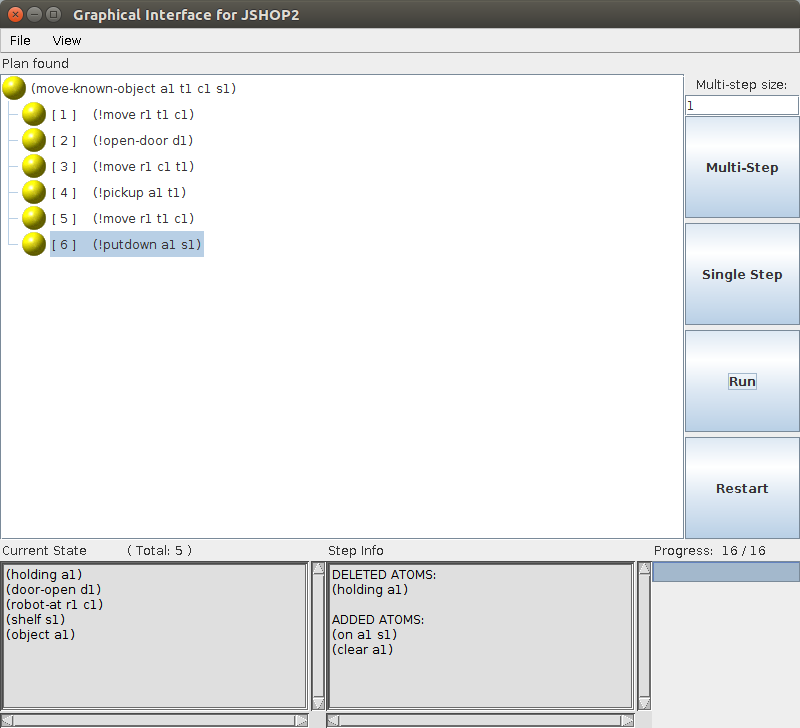
\includegraphics[width=0.65\linewidth]{images/problem1_gui}
		\caption{GUI Problem 1 }
		\label{fig:probem1_gui}
	\end{figure}

	\begin{figure}[h!]
	\centering
	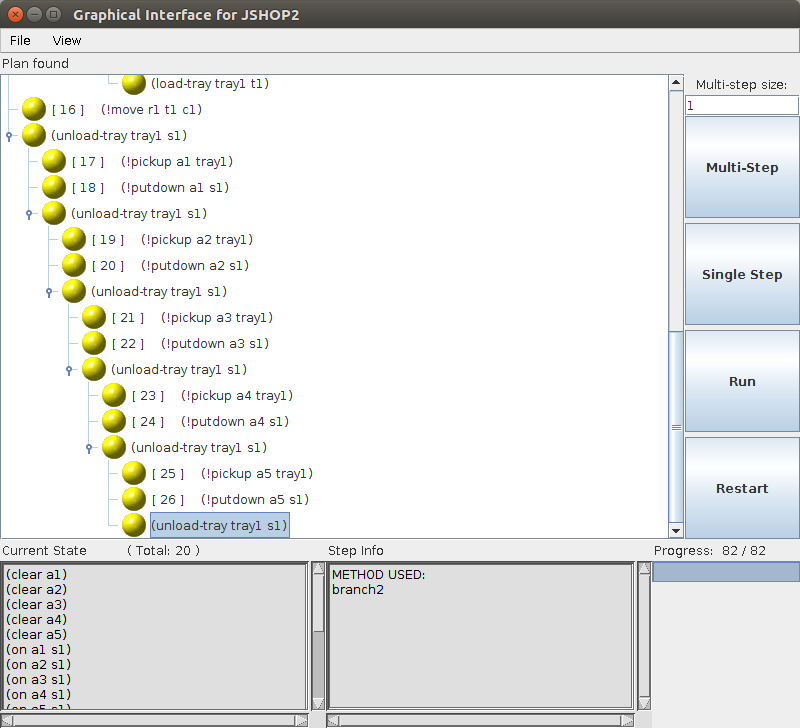
\includegraphics[width=0.65\linewidth]{images/problem2_gui}
	\caption{GUI Problem 2}
	\label{fig:problem2_gui}
	\end{figure}


	\begin{figure}[h!]
	\centering
	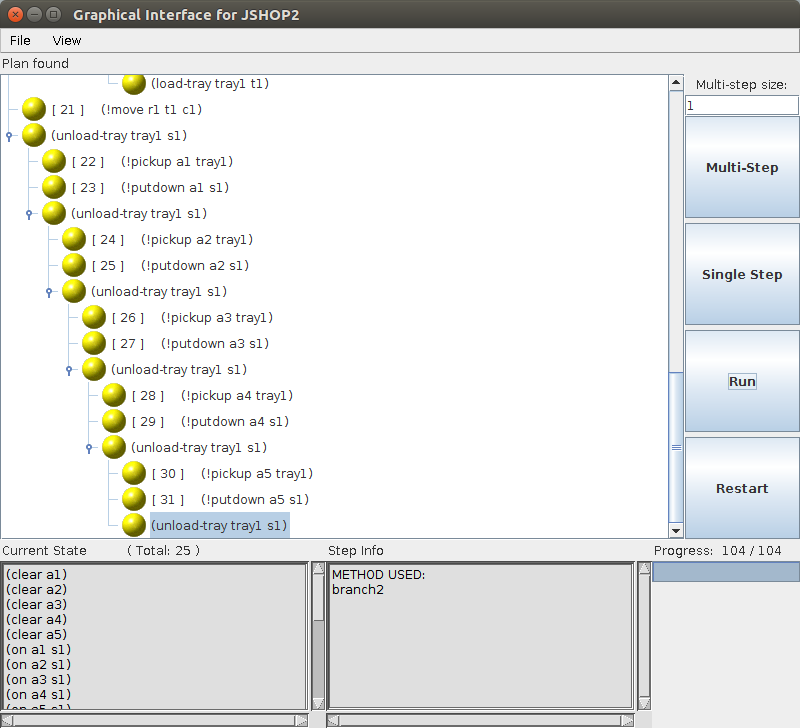
\includegraphics[width=0.65\linewidth]{images/problem3_gui}
	\caption{GUI Problem 3}
	\label{fig:problem3_gui}
	\end{figure}

	\begin{figure}[h!]
	\centering
	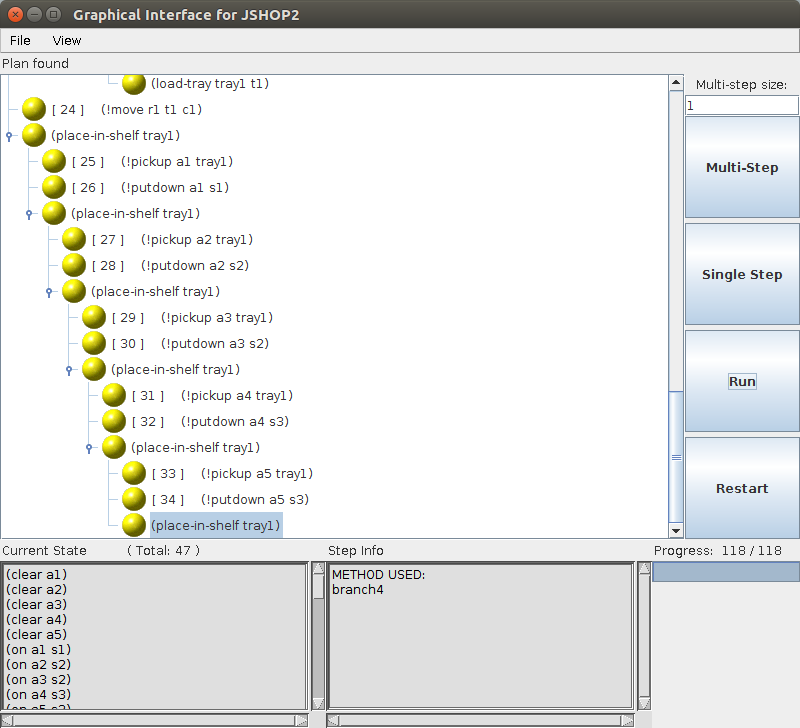
\includegraphics[width=0.65\linewidth]{images/problem4_gui}
	\caption{GUI Problem 4}
	\label{fig:problem4_gui}
	\end{figure}


	\newpage

	\section{Limitations and Planning Failures} \label{sec:limitations}

	The planner will fail if the initial state does not fulfill the assumptions described in section \ref{sec:assumptions}. Here we present some examples where the planner fails.

	\subsection{The planner does not have enough information for classifying an object.}


	In problem 4, the planner classifies all the objects based on their properties. The initial state includes properties for each object, like $is-round$ or $is-can$. The axioms in the problem domain are used for classifying objects. For instance, an object is classified as a drink if it is a bottle or a can. \\

	\begin{lstlisting}
; Characteristics of a drink
	(:- (is-drink ?a)
	(or (is-bottle ?a)(is-can ?a))
)
	\end{lstlisting}

	\vspace{5mm}

	The primitive task $!label-object ?a$ labels an object. If the precondition $is-drink ?a$ is met, the object is labeled as a drink. \\

	\begin{lstlisting}
;; To label an object as a drink
(:operator (!label-object ?a)
	((is-drink ?a))
	nil
	((drink-label ?a)(labeled ?a)))
	\end{lstlisting}

	\vspace{5mm}

	The method $label-objects$ is called recursively until all objects are labeled. \\

	\begin{lstlisting}
 ;; To label the objects
 (:method (label-objects)
	 branch1
	 (forall (?z) ((object ?z))(labeled ?z))
	 nil

	 branch2
	 ((object ?z)(not (labeled ?z)))
	 ((!label-object ?z)(label-objects))
 )
	\end{lstlisting}

	\vspace{5mm}

	If the information needed for classifying an object is missing from the problem definition, the object will no be classified and the planner will get stuck in the recursion of the method $label-objects$. \\

	Figure \ref{fig:failure-1} shows the output of the planner when 6 objects are in the problem definition and the information for classifying one of them is missing. The planner runs 17715 steps but fails to return a plan because the information about object $a4$ is missing. All objects should be labeled to stop the recursion. Since this condition is never met, the plan fails. \\

	The problem definition for this case is as follows: \\

	\begin{lstlisting}
(defproblem problem4 storegroceries
	;;Case4
	(
		(object a1)
		(object a2)
		(object a3)
		(object a4)
		(object a5)
		(object a6)
		(camera camera1)
		(cupboard c1)
		(door d1)
		(shelf s1)
		(shelf s2)
		(shelf s3)
		(table t1)
		(robot r1)
		(tray tray1)

		(unknown-location t1)(unknown-location c1)(unlabeled c1)
		(holds-snack s1)
		(holds-drink s2)
		(holds-fruit s3)
		(on a1 t1)(is-bag a1)(is-crunchy a1)
		(on a2 t1)(is-bottle a2)
		(on a3 t1)(is-can a3)
		;; (on a4 t1)(is-can a4)  <- object 4 does not have complete information
		(on a5 t1)(is-round a5)
		(on a6 t1)(is-bag a6)(is-crunchy a6)
		(door-closed d1)(robot-at r1 t1)
	)
	((move-unlabeled-object-unknown-cupboard t1 c1 s1 tray1 camera1))
)
	\end{lstlisting}

	\vspace{5mm}


	The error message shows that the planner gets stuck in a backtracking process. \\

	\begin{lstlisting}
Exception in thread "AWT-EventQueue-0" java.lang.ArrayIndexOutOfBoundsException: -1
at java.util.ArrayList.elementData(ArrayList.java:422)
at java.util.ArrayList.get(ArrayList.java:435)
at JSHOP2.JSHOP2GUI.processBacktracking(JSHOP2GUI.java:764)
at JSHOP2.JSHOP2GUI.runOneStep(JSHOP2GUI.java:512)
at JSHOP2.JSHOP2GUI.access$100(JSHOP2GUI.java:16)
...
	\end{lstlisting}



\subsection{A shelf does not hold an object in the initial state.}

In problem 4, the robot labels the shelfs based on the initial object that each shelf holds. If a shelf is empty, the robot will not be able to label it and the planner will get stuck in a recursive method. This problem is similar to the one discussed in the previous section. The method $explore-cupboard$ is called recursively until all shelfs are labeled. If the program does not have enough information for labeling all shelfs, the planner will fail. \\

\begin{lstlisting}

;; To explore the shelves of the cupboard ?c
	(:method (explore-cupboard ?c)
		branch1
		(forall (?z) ((shelf ?z))(labeled ?z))
		nil

		branch2
		((shelf ?z)(not (labeled ?z)))
		((!label-shelf ?z)(explore-cupboard ?c))
)
\end{lstlisting}

\vspace{5mm}

The problem definition for this case is as follows: \\

\begin{lstlisting}
(defproblem problem4 storegroceries
	;;Problem4
	(
		(object a1)
		(object a2)
		(object a3)
		(object a4)
		(object a5)
		(camera camera1)
		(cupboard c1)
		(door d1)
		(shelf s1)
		(shelf s2)
		(shelf s3)
		(table t1)
		(robot r1)
		(tray tray1)

		(unknown-location t1)(unknown-location c1)(unlabeled c1)
		;;(holds-snack s1) <- Shelf 1 does not hold an object
		(holds-drink s2)
		(holds-fruit s3)
		(on a1 t1)(is-bag a1)(is-crunchy a1)
		(on a2 t1)(is-bottle a2)
		(on a3 t1)(is-can a3)
		(on a4 t1)(is-round a4)
		(on a5 t1)(is-round a5)
		(door-closed d1)(robot-at r1 t1)
	)
	((move-unlabeled-object-unknown-cupboard t1 c1 s1 tray1 camera1))
)

\end{lstlisting}

\vspace{5mm}

Figure \ref{fig:failure-2} shows that the planner fails after 60 steps.

\begin{figure} [ht!]
	\centering
	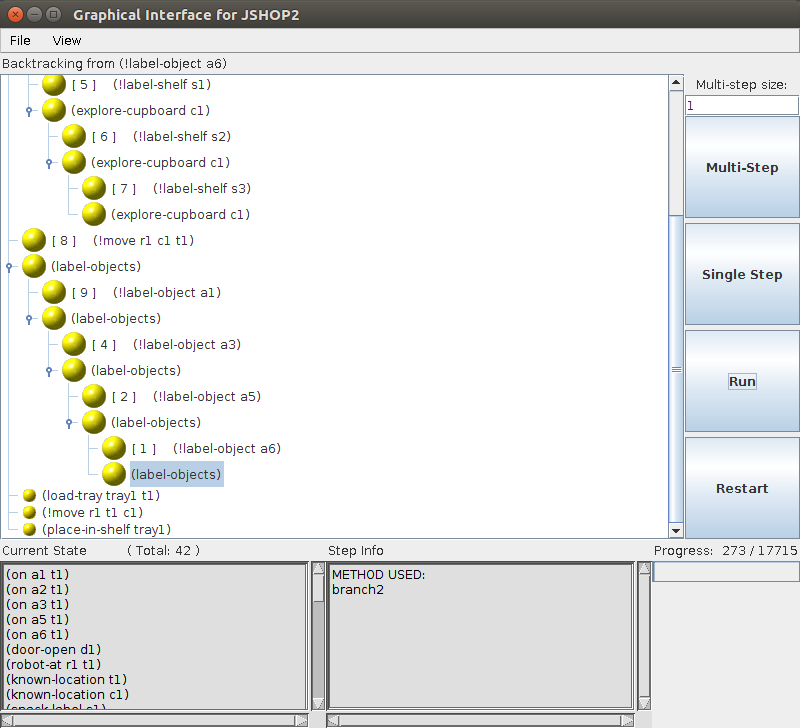
\includegraphics[width=0.65\linewidth]{images/failure-1}
	\caption{Failure: The planner does not have enough information for classifying an object.}
	\label{fig:failure-1}
\end{figure}


\begin{figure} [h!]
	\centering
	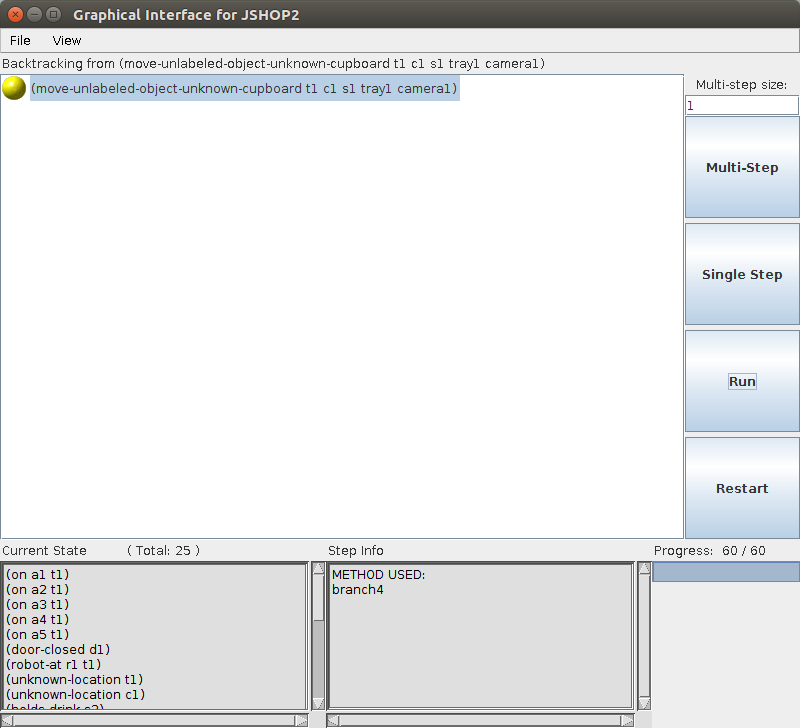
\includegraphics[width=0.65\linewidth]{images/failure-2}
	\caption{Failure: A shelf does not hold an object in the initial state.}
	\label{fig:failure-2}
\end{figure}


\subsection{The problem definition is compiled using java -ra}

The problem descriptions can be compiled into java bytecode using the commands documented in \cite{Ilghami2006}, like for example:

 \begin{itemize}
 	\item java JSHOP2.InternalDomain -r InputFileName
 	\item java JSHOP2.InternalDomain -rSomeInteger InputFileName
 	\item java JSHOP2.InternalDomain -ra InputFileName
 \end{itemize}

 If the option -r is used, the planner returns the first plan that it finds, in combination with a (-ra) all possible plans are returned. With -rSomeInteger the number of plans which are to be explored can be defined. \\

 Initially, we compiled our problem definitions using the -ra command, as it is shown in many of the jshop2 examples, but since we have an exponential growth in memory consumption, including more than 4 objects in the problem definition leads to OutOfMemoryError on our machines. \\


\begin{lstlisting}
Exception in thread "Thread-0" java.lang.OutOfMemoryError: GC overhead limit exceeded
at JSHOP2.State.iterator(State.java:227)
at JSHOP2.PreconditionAtomic.resetHelper(PreconditionAtomic.java:62)
at JSHOP2.Precondition.reset(Precondition.java:126)
at Precondition16.resetHelper(storegroceries.java:2357)
at JSHOP2.Precondition.reset(Precondition.java:126)
at Precondition17.resetHelper(storegroceries.java:2432)
at JSHOP2.Precondition.reset(Precondition.java:126)

\end{lstlisting}

\vspace{5mm}

We changed the compile option to -r and were able to get plans for $n$ objects (where $n= 1, 2, 3, 4, 5$) as shown in Table \ref{table:n-objects}. We have tested our solution for problem 4 with up to 20 objects. The resulting plan has 358 steps and its is accomplished using 109 primitive tasks: \\

\begin{lstlisting}

[ 1 ]    (!locate t1)
[ 2 ]    (!locate c1)
[ 3 ]    (!move r1 t1 c1)
[ 4 ]    (!open-door d1)
[ 5 ]    (!label-shelf s1)
[ 6 ]    (!label-shelf s2)
[ 7 ]    (!label-shelf s3)
[ 8 ]    (!move r1 c1 t1)
[ 9 ]    (!label-object a1)
[ 10 ]    (!label-object a2)
[ 11 ]    (!label-object a3)
[ 12 ]    (!label-object a4)
[ 13 ]    (!label-object a5)
[ 14 ]    (!label-object a6)
[ 15 ]    (!label-object a7)
[ 16 ]    (!label-object a8)
[ 17 ]    (!label-object a9)
[ 18 ]    (!label-object a10)
[ 19 ]    (!label-object a11)
[ 20 ]    (!label-object a12)
[ 21 ]    (!label-object a13)
[ 22 ]    (!label-object a14)
[ 23 ]    (!label-object a15)
[ 24 ]    (!label-object a16)
[ 25 ]    (!label-object a17)
[ 26 ]    (!label-object a18)
[ 27 ]    (!label-object a19)
[ 28 ]    (!label-object a20)
[ 29 ]    (!pickup a1 t1)
[ 30 ]    (!putdown a1 tray1)
[ 31 ]    (!pickup a2 t1)
[ 32 ]    (!putdown a2 tray1)
[ 33 ]    (!pickup a3 t1)
[ 34 ]    (!putdown a3 tray1)
[ 35 ]    (!pickup a4 t1)
[ 36 ]    (!putdown a4 tray1)
[ 37 ]    (!pickup a5 t1)
[ 38 ]    (!putdown a5 tray1)
[ 39 ]    (!pickup a6 t1)
[ 40 ]    (!putdown a6 tray1)
[ 41 ]    (!pickup a7 t1)
[ 42 ]    (!putdown a7 tray1)
[ 43 ]    (!pickup a8 t1)
[ 44 ]    (!putdown a8 tray1)
[ 45 ]    (!pickup a9 t1)
[ 46 ]    (!putdown a9 tray1)
[ 47 ]    (!pickup a10 t1)
[ 48 ]    (!putdown a10 tray1)
[ 49 ]    (!pickup a11 t1)
[ 50 ]    (!putdown a11 tray1)
[ 51 ]    (!pickup a12 t1)
[ 52 ]    (!putdown a12 tray1)
[ 53 ]    (!pickup a13 t1)
[ 54 ]    (!putdown a13 tray1)
[ 55 ]    (!pickup a14 t1)
[ 56 ]    (!putdown a14 tray1)
[ 57 ]    (!pickup a15 t1)
[ 58 ]    (!putdown a15 tray1)
[ 59 ]    (!pickup a16 t1)
[ 60 ]    (!putdown a16 tray1)
[ 61 ]    (!pickup a17 t1)
[ 62 ]    (!putdown a17 tray1)
[ 63 ]    (!pickup a18 t1)
[ 64 ]    (!putdown a18 tray1)
[ 65 ]    (!pickup a19 t1)
[ 66 ]    (!putdown a19 tray1)
[ 67 ]    (!pickup a20 t1)
[ 68 ]    (!putdown a20 tray1)
[ 69 ]    (!move r1 t1 c1)
[ 70 ]    (!pickup a1 tray1)
[ 71 ]    (!putdown a1 s1)
[ 72 ]    (!pickup a6 tray1)
[ 73 ]    (!putdown a6 s1)
[ 74 ]    (!pickup a11 tray1)
[ 75 ]    (!putdown a11 s1)
[ 76 ]    (!pickup a16 tray1)
[ 77 ]    (!putdown a16 s1)
[ 78 ]    (!pickup a2 tray1)
[ 79 ]    (!putdown a2 s2)
[ 80 ]    (!pickup a3 tray1)
[ 81 ]    (!putdown a3 s2)
[ 82 ]    (!pickup a7 tray1)
[ 83 ]    (!putdown a7 s2)
[ 84 ]    (!pickup a8 tray1)
[ 85 ]    (!putdown a8 s2)
[ 86 ]    (!pickup a12 tray1)
[ 87 ]    (!putdown a12 s2)
[ 88 ]    (!pickup a13 tray1)
[ 89 ]    (!putdown a13 s2)
[ 90 ]    (!pickup a17 tray1)
[ 91 ]    (!putdown a17 s2)
[ 92 ]    (!pickup a18 tray1)
[ 93 ]    (!putdown a18 s2)
[ 94 ]    (!pickup a4 tray1)
[ 95 ]    (!putdown a4 s3)
[ 96 ]    (!pickup a5 tray1)
[ 97 ]    (!putdown a5 s3)
[ 98 ]    (!pickup a9 tray1)
[ 99 ]    (!putdown a9 s3)
[ 100 ]    (!pickup a10 tray1)
[ 101 ]    (!putdown a10 s3)
[ 102 ]    (!pickup a14 tray1)
[ 103 ]    (!putdown a14 s3)
[ 104 ]    (!pickup a15 tray1)
[ 105 ]    (!putdown a15 s3)
[ 106 ]    (!pickup a19 tray1)
[ 107 ]    (!putdown a19 s3)
[ 108 ]    (!pickup a20 tray1)
[ 109 ]    (!putdown a20 s3)

\end{lstlisting}

\vspace{5mm}

The domain for solving problems 1 to 4 works under the assumptions described in section \ref{sec:assumptions}. If one of these assumptions is not met, the planner will fail. Modifications can be made to increase the flexibility of the domain. For instance, if the robot is not at the table, it is possible to include a task for localizing and moving the robot to the table. If the shelf does not contain an object, one could assign a label to it based on the object categories.

	\bibliography{bibliography}{}
	\bibliographystyle{plain}


\end{document}
